\documentclass[10pt, a4paper]{article}
\usepackage[margin=0.75in]{geometry}
\usepackage{graphicx}
\usepackage{wrapfig}
\usepackage{caption}
\usepackage{subcaption}
\usepackage{hyperref}
\graphicspath{{images/}}

\title{Applied Machine Learning - Exploratory Sentiment Analysis}
\author{Poppy Z Grimes, Pinar Batat Buke, Zhifan Sun}
\date{November 2022}


\begin{document}
\maketitle 

\section{Task description}

Sentiment analysis is an important method within the sphere of natural language processing (NLP) to classify the positive or negative feeling within human text or speech. In the context of machine learning algorithms, sentiment analysis can be performed using both supervised and unsupervised methods. 

This project presents an exploratory analysis on the Stanford Sentiment Treebank (SST-5) dataset. We apply and build various task-based and feature-based algorithms and assess their performance in determining sentiment of online film reviews. We approach this by testing both full sentences and phrases. In addition, we explore how various pre-processing techniques effect our outcomes. This includes lemmetisation, human subjectivity etc. %edit here

Our primary aim is to build a model that can predict sentiment of sentences in the SST-5 dataset. To do this we will explore various algorithms and identify the one with the highest accuracy. Our work will compare outputs with previous work.
%compared with human based classifier?

Our secondary aim is to discuss the effect of data-preprocessing and formatting on the analysis. Methods incorporated include lemmetisation...


\section{Background and related work}
The SST-5 dataset is a repository of x %number?
film reviews from RottenTomatoes.com. The repository is organised into several files which split the data into sentences or phrases. Phrases from reviews have human-assigned sentiment scores where participants were asked to score on a continuous sliding scale seen in figure \ref{fig:sentiment_scale}.

\begin{wrapfigure}{l}{0.3\textwidth}
    \begin{center}
        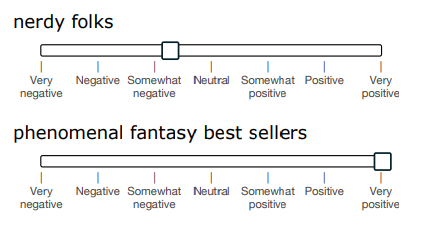
\includegraphics[width=0.189\textwidth]{sentiment_scale} 
    \end{center}
\caption{Continuous sentiment scale}
\label{fig:sentiment_scale}
\end{wrapfigure}

From this, phrases were assigned into one of five sentiment classes, producing a fine-grained sentiment labelled dataset. Unlike binary data, having five discrete classes overcomes the limitation of binary classifiers when faced with dual polarity (cite). A noteworthy example of this can be seen in negation \textit{e.g. 'this film hardly made me laugh'}. 

\subsection{Training on a recursive Neural Tensor Network (RNTN)}
This dataset was initially introduced by Socher \textit{et al.} (2013) to test a new neural network model with the aim to outperform previous algorithms on a) binary classification and b) fine-grained sentiment labels.

We also identified an analysis by Rao (2019) who took a similar approach to us in attempting to classify whole-sentences

\subsection{Bag of words (BOW)}
Bag of words is a popular method which tracks the polarity of individual words. It can be used to weight particularly positive or negative individual words accordingly. As a result, it is more successful in longer text strings. BOW exhibits weakness in that it does not account for grammatical, semantic or structural features within language. We decided to implement this as a baseline comparison but with the expectation of low performance.









\section{Task significance}











\section{Information on Data Pre-processing}

\subsection{Phrase pre-processing steps}

\begin{enumerate} 
    \item Align each phrase with its label using the phrase ID by combining dictionary.txt and sentiment\_labels.txt
    \item Classify labels into discrete bins from the range [0,1] into classes ranging from 1 to 5
    \item Lemmetisation
    \begin{enumerate}
        \item Using \textit{Stanza} library get lemma of each word in phrases returning either verb, adjective, adverb
        \item Also select for word "not" in each phrase (negation)
        \item Using \textit{NLTK} library remove stop words 
    \end{enumerate}
    \item Create a dataframe with columns: $['id', 'phrase', 'lemma', 'key\_words', 'label'],$ where $key\Uwords$ column contain the verbs, adjective and adverb of each phrase.
\end{enumerate}
    
    
    
    

\subsection{Sentence pre-processing}

\subsubsection{Assigning sentiment scores to sentences}
The provided data set assigns sentiment scores only to individual phrases, or n-grams. For the purpose of our supervised analysis, we need sentiment labels for full sentences. The first method we have chosen is to manually score (human-based) a random sample of n=100 sentences as positive or negative. This will be a test dataset.

A second method we explore is using the x function in NLTK library which generates a portfolio of scores for each datapoint for positive, neutral and negative. From this we compute a compound score in the range [0,1]. 




Second, we have pulled positive and negative words with high polarity with assigned sentiment from the labelled phrase-bank. For both routes, these will act as labels for training our classifiers. 










\section{Exploratory data analysis}

\subsection{Phrase Analysis}
\subsubsection{Word Clouds}
We drew word cloud images for each class, and for both the lemma data and the key\_word data. Keywords appear to be more relevant with the label Figures \ref{fig:classcloud} and \ref{fig:lemmacloud}.

\begin{figure}[h]
     \centering
     \begin{subfigure}[b]{0.18\textwidth}
         \centering
         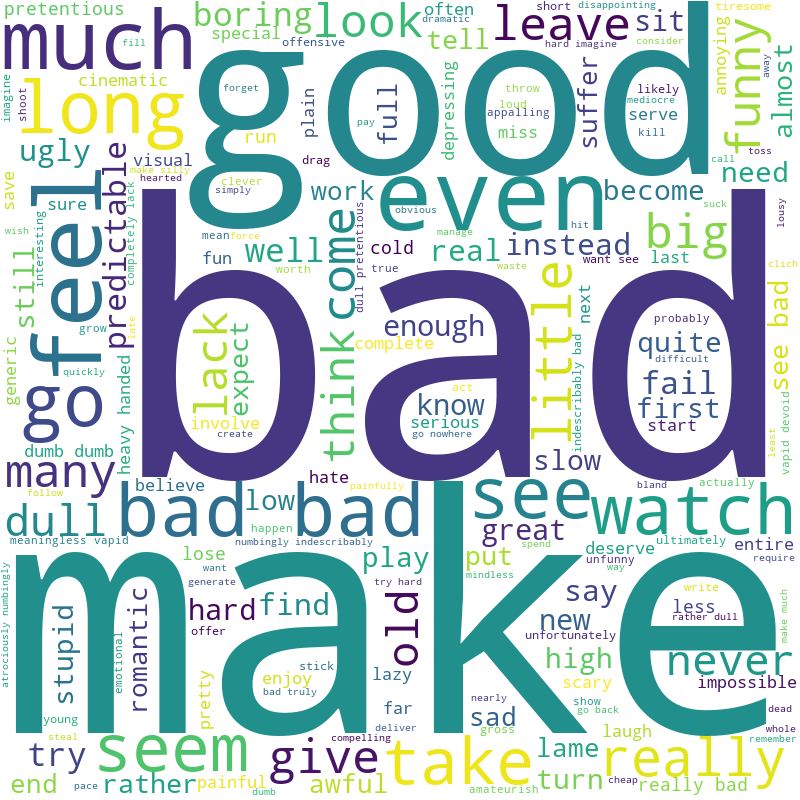
\includegraphics[width=\textwidth]{keywords1.png}
         \caption{Class 1}
         \label{fig:class1cloud}
     \end{subfigure}
     \hfill
     \begin{subfigure}[b]{0.18\textwidth}
         \centering
         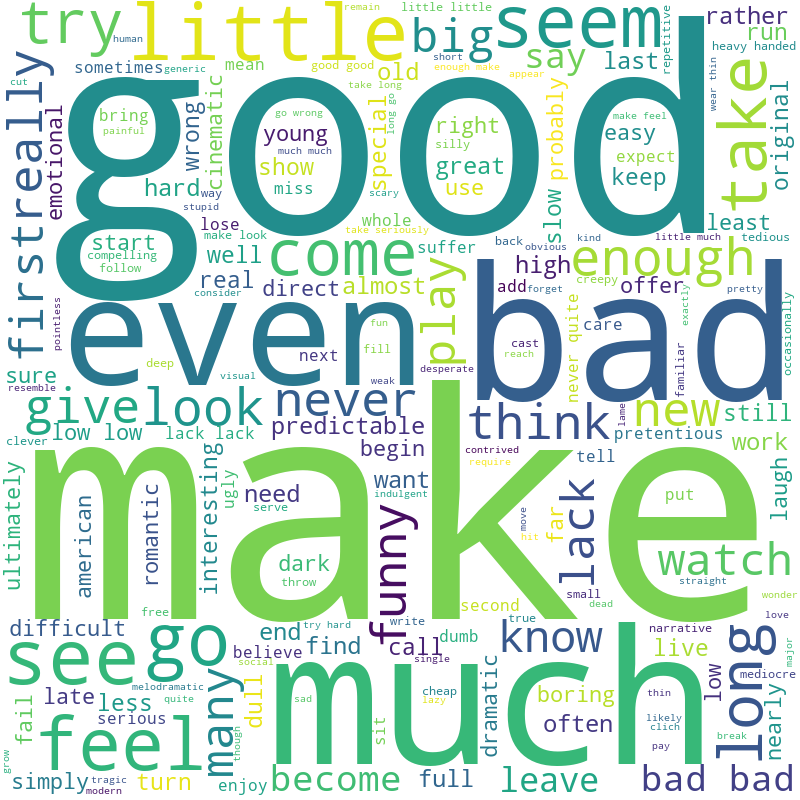
\includegraphics[width=\textwidth]{keywords2.png}
         \caption{Class 2}
         \label{fig:class2cloud}
     \end{subfigure}
     \hfill
     \begin{subfigure}[b]{0.18\textwidth}
         \centering
         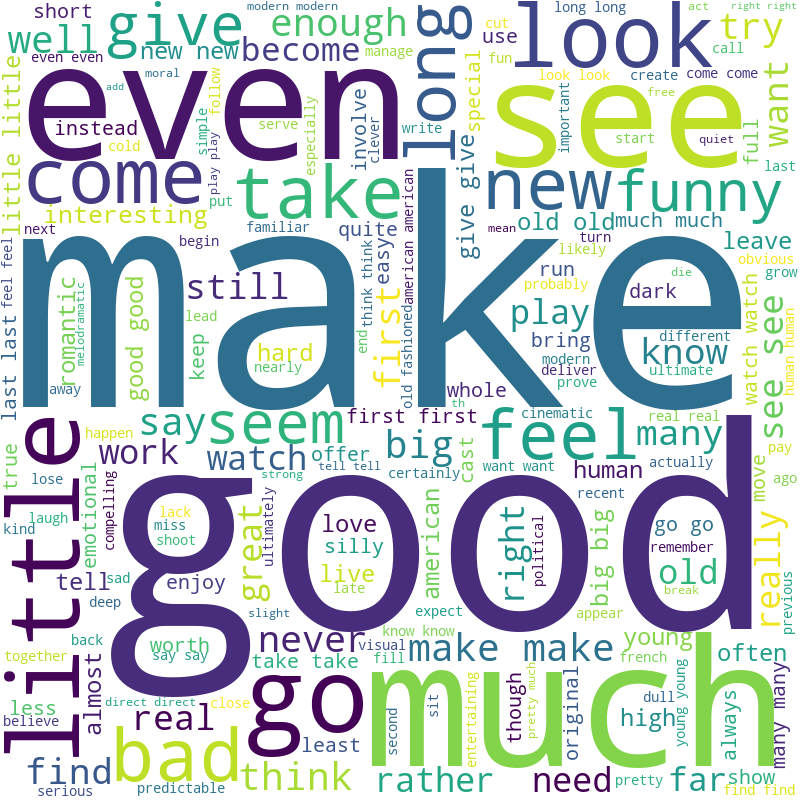
\includegraphics[width=\textwidth]{keywords3.png}
         \caption{Class 3}
         \label{fig:class3cloud}
     \end{subfigure}
     \hfill
     \begin{subfigure}[b]{0.18\textwidth}
         \centering
         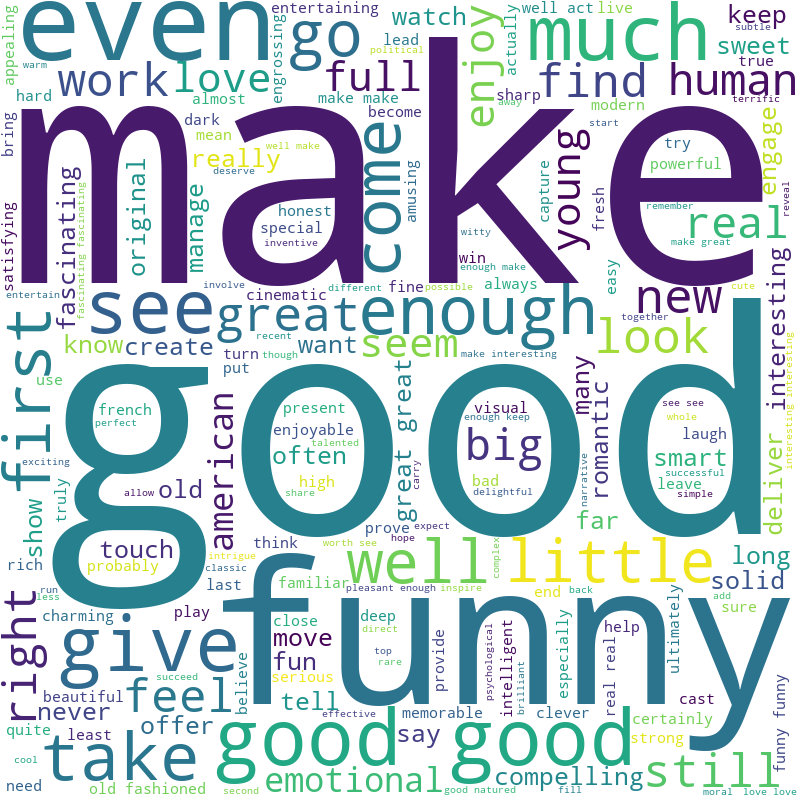
\includegraphics[width=\textwidth]{keywords4.png}
         \caption{Class 4}
         \label{fig:class4cloud}
     \end{subfigure}
     \hfill
     \begin{subfigure}[b]{0.18\textwidth}
         \centering
         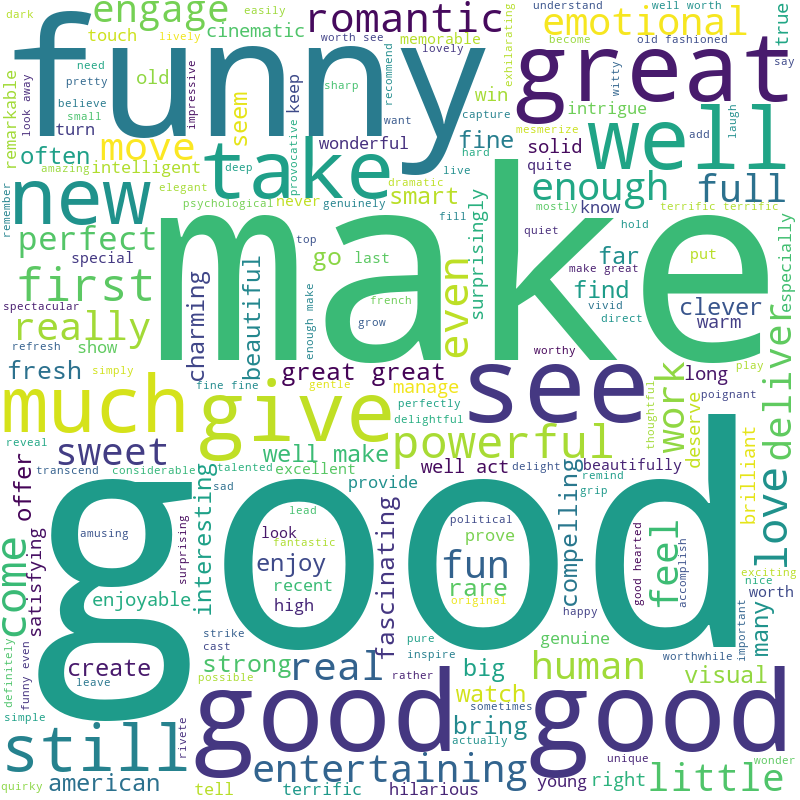
\includegraphics[width=\textwidth]{keywords5.png}
         \caption{Class 5}
         \label{fig:class5cloud}
     \end{subfigure}
     \hfill
    \caption{Word clouds for keywords in each class}
\label{fig:classcloud}
\end{figure}
\begin{figure}[h]
     \centering
     \begin{subfigure}[b]{0.18\textwidth}
         \centering
         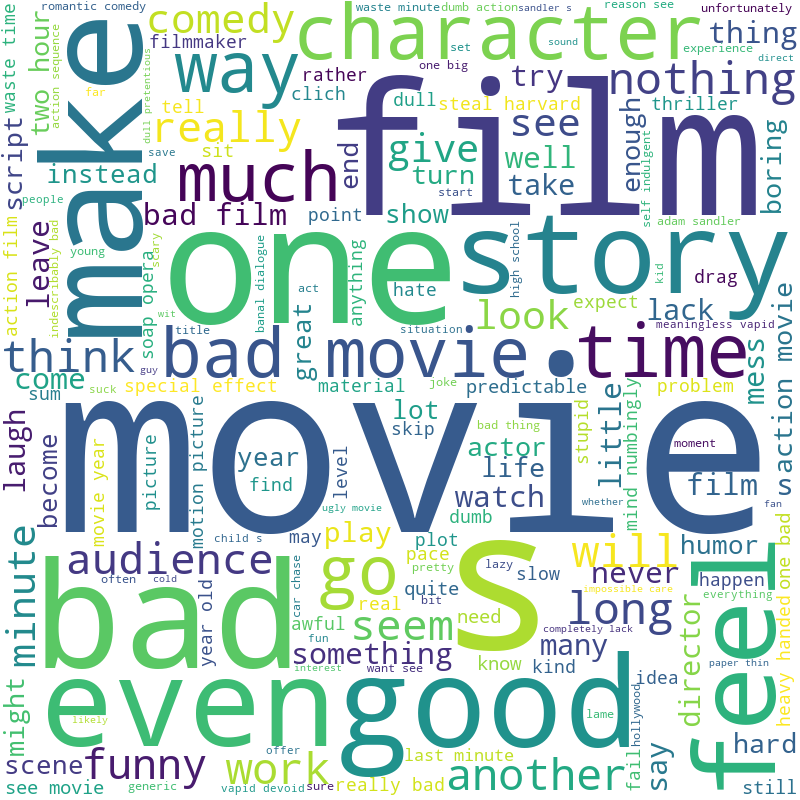
\includegraphics[width=\textwidth]{lemma1.png}
         \caption{Class 1}
         \label{fig:lemma1cloud}
     \end{subfigure}
     \hfill
     \begin{subfigure}[b]{0.18\textwidth}
         \centering
         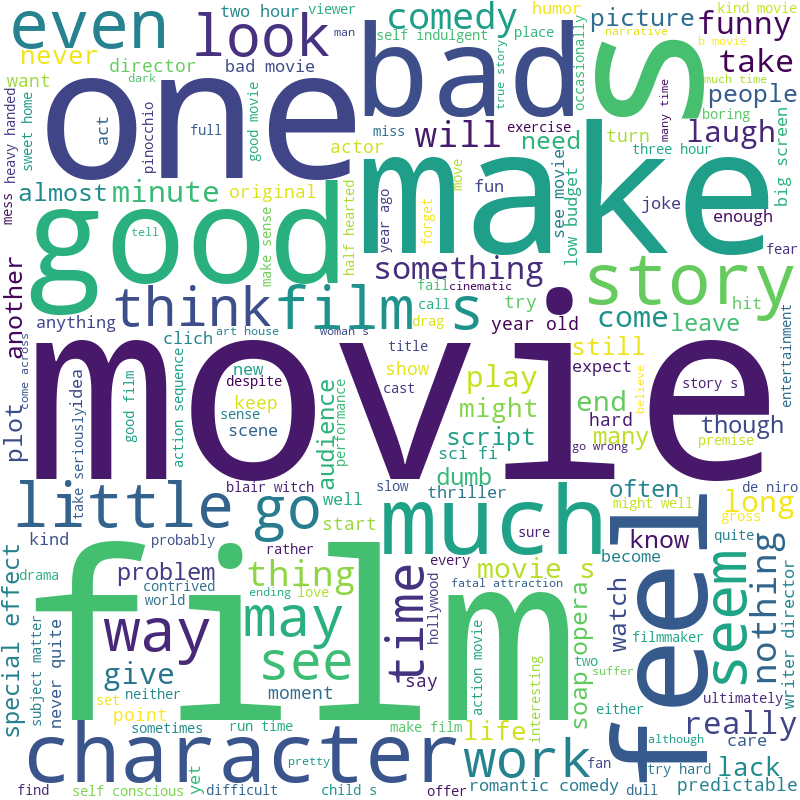
\includegraphics[width=\textwidth]{lemma2.png}
         \caption{Class 2}
         \label{fig:lemma2cloud}
     \end{subfigure}
     \hfill
     \begin{subfigure}[b]{0.18\textwidth}
         \centering
         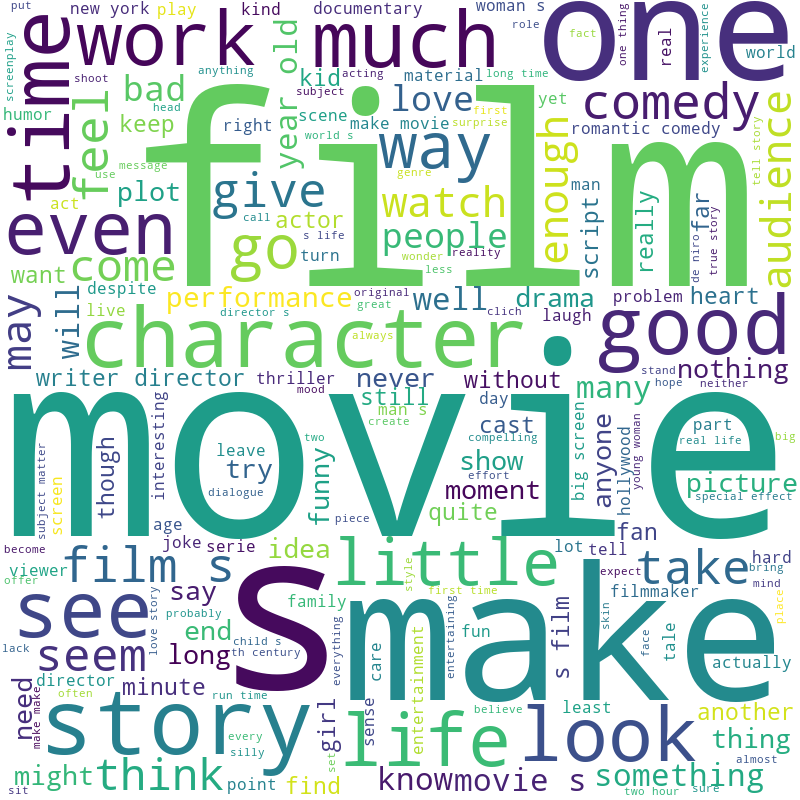
\includegraphics[width=\textwidth]{lemma3.png}
         \caption{Class 3}
         \label{fig:lemma3cloud}
     \end{subfigure}
     \hfill
     \begin{subfigure}[b]{0.18\textwidth}
         \centering
         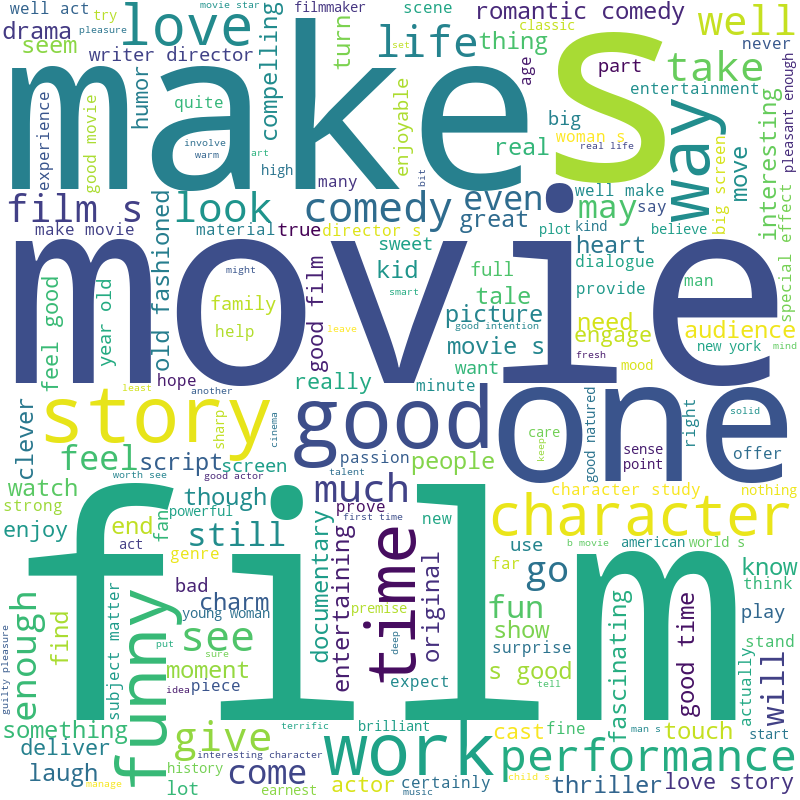
\includegraphics[width=\textwidth]{lemma4.png}
         \caption{Class 4}
         \label{fig:lemma4cloud}
     \end{subfigure}
     \hfill
     \begin{subfigure}[b]{0.18\textwidth}
         \centering
         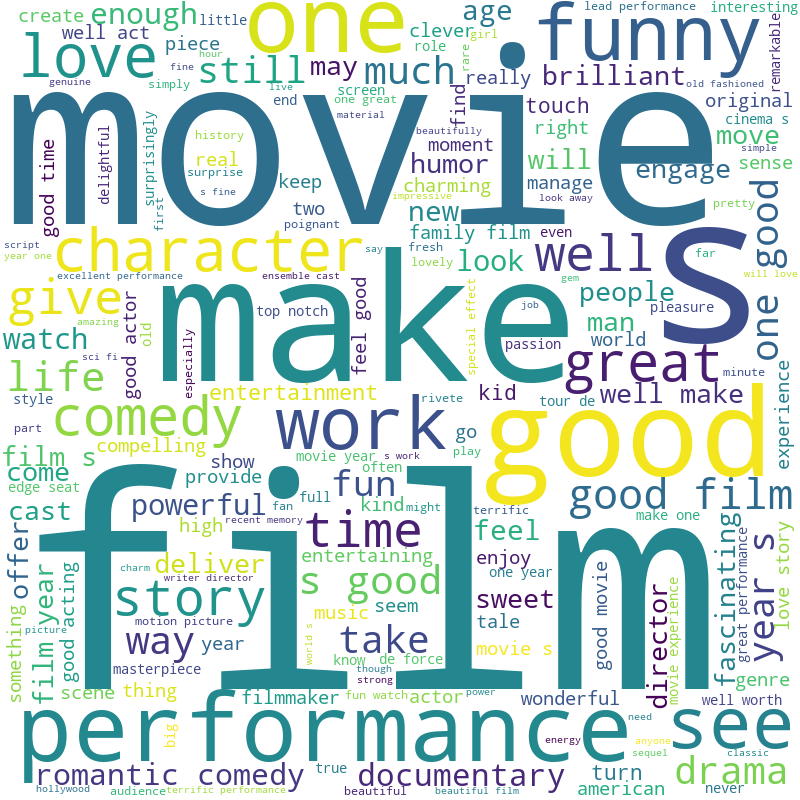
\includegraphics[width=\textwidth]{lemma5.png}
         \caption{Class 5}
         \label{fig:lemma5cloud}
     \end{subfigure}
     \hfill
    \caption{Word clouds for lemma in each class}
\label{fig:lemmacloud}
\end{figure}

To choose our input features we selected the 16 most frequent words from each class and additionally hand-picked 15 from the word-clouds. This brought us to a total of 95 keyword features. We performed supervised classification using three classes (positive, neutral and negative).


\subsection{Sentence Analysis}
We use an \href{http://ai.stanford.edu/~amaas/data/sentiment/}{external dataset} \cite{maas2011learning} to train our model for the sentence-based analysis as sentences are unlabelled in the SST-5 and we only had capacity on this occasion to hand-label 100. Our training dataset is from the IMDB movie review platform with n = 25,000 datapoints (sentences) labelled as positive or negative, following the same structure and inputs of our test data. We initially split the IMDB data into test (80\%) and train (20\%) before testing with the SST-5 data.




\section{Description of learning methods used}

Supervised training models
\begin{itemize}
    \item Naive Bayes'
    \item Logistic Regression
    \item Decision Tree
    \item Random Forest
\end{itemize}\\\


Unsupervised training models
\begin{itemize}
    \item Clustering
\end{itemize}

\section{Results and evaluation}

\subsection{Performance on sentences}

\subsubsection{Using human-based labelling}

\begin{table}[h]
\begin{center}
\begin{tabular}{||c c c c||} 
 \hline
 Classifier & Accuracy & Col3 & col4 \\ [0.5ex] 
 \hline\hline
 Naive Bayes' & x & x & x \\ 
 \hline 
 Logistic Regression & x & x & x \\
 \hline
 Decision Tree & 545 & 778 & 7507 \\
 \hline
 Random Forest & 545 & 18744 & 7560 \\
 \hline\hline
\end{tabular}
\caption{Results: Unsupervised learning of sentence}
\label{table:1}
\end{center}
\end{table}

\subsubsection{Using NLTK compound scores}


\section{Conclusions}



\bibliographystyle{plain}
\bibliography{bibliography}

\end{document}